\begin{frame}
\frametitle{Sumário}
\tableofcontents
\end{frame}

\section{Introdução e Definição do Problema}

% SLIDE 2: O GANCHO
\begin{frame}
\frametitle{Qual é o melhor caminho?}

\begin{columns}[T]
    \begin{column}{0.6\textwidth}
        \begin{block}{A Pergunta Intuitiva}
        Como o Google Maps sabe a rota mais rápida para chegar na FCT?
        \end{block}
        \begin{itemize}
            \item É o caminho mais rápido (menor tempo)?
            \item É o caminho mais curto (menor distância)?
            \item É o caminho mais barato (sem pedágios)?
        \end{itemize}
        \vspace{0.5cm}
        A ideia central é modelar o mapa como um \textbf{grafo} e atribuir \textbf{custos} às ruas.
    \end{column}

    \begin{column}{0.4\textwidth}
        \centering
        % Espaço reservado para a imagem.
        % Quando tiver a imagem, descomente a linha abaixo:
        \includegraphics[width=\linewidth]{images/googlemaps.png}
    \end{column}
\end{columns}
\end{frame}

% SLIDE 3: APLICAÇÕES PRÁTICAS
\begin{frame}
\frametitle{Onde o PCM se Esconde?}
\begin{itemize}
    \item \textbf{Redes de Computadores:} Roteamento de pacotes na internet (Protocolo OSPF) — o custo é a latência.
    \item \textbf{Logística e Transporte:} Otimização de rotas de entrega (Correios, Mercado Livre) — o custo é a distância ou tempo.
    \item \textbf{Finanças (Avançado):} Detecção de oportunidades de arbitragem em mercados (encontrar ciclos de custo negativo).
    \item \textbf{Análise de Redes Sociais:} Medir o "grau de separação" entre duas pessoas.
\end{itemize}
\end{frame}

% SLIDE 4: DEFINIÇÃO FORMAL - PARTE 1
\begin{frame}
\frametitle{Traduzindo o Mapa para a Matemática}

\begin{columns}[T]
    \begin{column}{0.6\textwidth}
        \begin{itemize}
            \item \textbf{Grafo (ou Dígrafo):} $G = (V, E)$
            \item \textbf{$V$ (Vértices):} O conjunto de "nós" (ex: cidades, roteadores).
            \item \textbf{$E$ (Arestas):} O conjunto de "conexões" (ex: ruas, cabos).
            \item \textbf{Grafo Ponderado:} Cada aresta $(i, j) \in E$ possui um \textbf{peso} (ou custo) $w_{ij}$ associado.
        \end{itemize}
    \end{column}

    \begin{column}{0.4\textwidth}
        \centering
        % Diagrama do Grafo usando TikZ (se não funcionar, avise)
        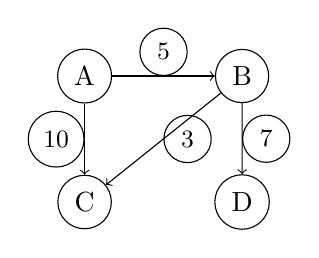
\begin{tikzpicture}[scale=0.8, every node/.style={circle, draw, minimum size=0.6cm}]
            \node (A) at (0,0) {A};
            \node (B) at (2.5,0) {B};
            \node (C) at (0,-2) {C};
            \node (D) at (2.5,-2) {D};
            \draw[->] (A) -- node[above, font=\small]{5} (B);
            \draw[->] (A) -- node[left, font=\small]{10} (C);
            \draw[->] (B) -- node[right, font=\small]{3} (C);
            \draw[->] (B) -- node[right, font=\small]{7} (D);
        \end{tikzpicture}
    \end{column}
\end{columns}
\end{frame}

% SLIDE 5: DEFINIÇÃO FORMAL - PARTE 2
\begin{frame}
\frametitle{O Problema de Caminhos Mínimos}

\begin{itemize}
    \item \textbf{Caminho:} Uma sequência de arestas que conecta um nó origem $s$ a um nó destino $t$.
    \begin{itemize}
        \item Ex: $P = (A \to B \to D)$
    \end{itemize}
    \item \textbf{Custo do Caminho:} A soma dos pesos $w_{ij}$ das arestas que formam o caminho.
    \begin{itemize}
        \item Ex: $Custo(P) = w_{AB} + w_{BD}$
    \end{itemize}
\end{itemize}
  
  % --- A CORREÇÃO É AQUI ---
  \begin{block}{O Grande Objetivo}
    Dado um grafo ponderado $G$, um nó origem $s$ e um nó destino $t$, encontrar o caminho $P$ de $s$ para $t$ que \textbf{minimiza o custo total}.
    \[
      P^* = \arg\min_{P:\, s\to t} \sum_{(i,j)\in P} w_{ij}
    \]
  \end{block}
  % --- FIM DA CORREÇÃO ---
  
  \begin{alertblock}{Observação Importante}
    Os algoritmos que vamos estudar (Dijkstra, Bellman-Ford) resolvem o problema de \textbf{Origem Única (SSSP)}: encontram o caminho mínimo de $s$ para \textbf{TODOS} os outros nós.
  \end{alertblock}
\end{frame}

% --- MÓDULO 2: MODELO MATEMÁTICO (PL) ---

\section{Modelo Matemático (PL)}

% SLIDE 6: VARIÁVEIS E FUNÇÃO OBJETIVO
\begin{frame}
\frametitle{Modelo PL: Variáveis e Função Objetivo}

\begin{block}{Variáveis de Decisão}
Definimos $x_{ij}$ como a quantidade de fluxo enviado pela aresta $(i, j)$.
\begin{itemize}
    \item $x_{ij} = 1$ se a aresta $(i, j)$ faz parte do caminho mínimo.
    \item $x_{ij} = 0$ caso contrário.
\end{itemize}
\end{block}

\begin{block}{Função Objetivo (Minimizar o Custo Total)}
Queremos minimizar a soma dos custos de todas as arestas usadas. O custo de usar a aresta $(i, j)$ é $w_{ij}$.
\[
\min Z = \sum_{(i,j) \in E} w_{ij} \cdot x_{ij}
\]
\end{block}
\end{frame}

% SLIDE 7: RESTRIÇÕES (PARTE 1)
\begin{frame}
\frametitle{Modelo PL: Restrições de Conservação de Fluxo}

Para cada nó $k$ no grafo, o fluxo que "entra" deve ser igual ao fluxo que "sai", com exceção da origem e do destino.

\vspace{0.5cm}

\textbf{1. Nó Origem ($s$):}
\begin{itemize}
    \item O nó $s$ \textbf{envia 1} unidade de fluxo.
    \item Fluxo que Sai - Fluxo que Entra = 1
    \[
    \sum_{j:(s,j) \in E} x_{sj} - \sum_{i:(i,s) \in E} x_{is} = 1
    \]
\end{itemize}

\vspace{0.5cm}

\textbf{2. Nó Destino ($t$):}
\begin{itemize}
    \item O nó $t$ \textbf{recebe 1} unidade de fluxo.
    \item Fluxo que Sai - Fluxo que Entra = -1
    \[
    \sum_{j:(t,j) \in E} x_{tj} - \sum_{i:(i,t) \in E} x_{it} = -1
    \]
\end{itemize}
\end{frame}

% SLIDE 8: RESTRIÇÕES (PARTE 2)
\begin{frame}
\frametitle{Modelo PL: Restrições de Conservação de Fluxo}

\textbf{3. Nós Intermediários ($k \neq s, t$):}
\begin{itemize}
    \item Tudo que entra deve sair (conservação pura).
    \item Fluxo que Sai - Fluxo que Entra = 0
    \[
    \sum_{j:(k,j) \in E} x_{kj} - \sum_{i:(i,k) \in E} x_{ik} = 0
    \]
\end{itemize}

\vspace{1cm}

\begin{block}{4. Restrição de Não-Negatividade}
Não podemos enviar fluxo negativo.
\[ 
x_{ij} \ge 0 \quad \forall (i,j) \in E 
\]
\end{block}
\end{frame}

% SLIDE 9: A MÁGICA DA PROGRAMAÇÃO LINEAR
\begin{frame}
\frametitle{Modelo PL: A Mágica da Integridade}

\begin{itemize}
    \item \textbf{Pergunta:} Nós não deveríamos forçar $x_{ij}$ a ser um número inteiro ($0$ ou $1$)?
    \[
    x_{ij} \in \{0, 1\} \quad \text{(Programação Inteira)}
    \]
    \item \textbf{Resposta:} Não precisa!
    \item Este tipo de problema de rede (Fluxo de Custo Mínimo) tem uma propriedade especial chamada \textbf{Total Unimodularidade}.
    \item \textbf{O que importa:} Essa propriedade \textbf{garante} que, se a oferta (1) e a demanda (-1) são inteiras, a solução ótima do problema de Programação Linear (com $x_{ij} \ge 0$) \textbf{já será inteira}.
    \item Por isso, podemos resolvê-lo eficientemente como um PL comum.
\end{itemize}
\end{frame}

% --- MÓDULO 3: MÉTODOS DE RESOLUÇÃO ---

\section{Métodos de Resolução}

% SLIDE 11: INTRODUÇÃO AOS ALGORITMOS
\begin{frame}
\frametitle{Módulo 3: Métodos de Resolução}

\begin{itemize}
    \item Embora o modelo de PL seja academicamente correto, ele não é a forma mais \textit{eficiente} de resolver o Problema de Caminhos Mínimos na prática.
    \item Na prática, usamos algoritmos especializados em grafos que são muito mais rápidos.
    \item Vamos focar em dois algoritmos fundamentais:
    \begin{enumerate}
        \item \textbf{Algoritmo de Dijkstra}
        \item \textbf{Algoritmo de Bellman-Ford}
    \end{enumerate}
\end{itemize}
\end{frame}

% SLIDE 12: ALGORITMO DE DIJKSTRA (CONCEITO)
\begin{frame}
\frametitle{Algoritmo de Dijkstra}

\begin{block}{O Conceito}
Uma abordagem "Gulosa" (Greedy). A cada passo, ele escolhe o caminho que \textit{parece} ser o melhor (o mais curto) e expande a partir dele.
\end{block}

\begin{alertblock}{Restrição Crítica}
O Algoritmo de Dijkstra \textbf{NÃO FUNCIONA} se o grafo tiver arestas com \textbf{pesos negativos}.
\end{alertblock}

\begin{itemize}
    \item \textbf{Ideia Principal:}
    \begin{itemize}
        \item Mantém um conjunto de nós "visitados" e as distâncias até eles.
        \item Começa na origem $s$ (distância 0) e todos os outros com distância $\infty$.
        \item Em cada passo, visita o nó \textbf{não-visitado} com a \textbf{menor distância} atual.
        \item Ao visitar um nó, "relaxa" as arestas para seus vizinhos (tenta encontrar um caminho mais curto para eles).
    \end{itemize}
\end{itemize}
\end{frame}

% SLIDE 13: ALGORITMO DE DIJKSTRA (EXEMPLO)
\begin{frame}
\frametitle{Exemplo Prático: Algoritmo de Dijkstra}

\begin{columns}[T]
    \begin{column}{0.4\textwidth}
        \centering
        % O mesmo diagrama que usamos antes
        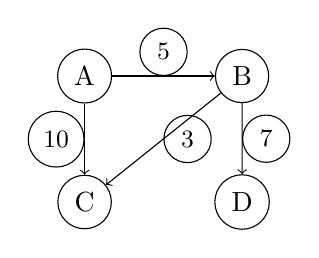
\begin{tikzpicture}[scale=0.8, every node/.style={circle, draw, minimum size=0.6cm}]
            \node (A) at (0,0) {A};
            \node (B) at (2.5,0) {B};
            \node (C) at (0,-2) {C};
            \node (D) at (2.5,-2) {D};
            \draw[->] (A) -- node[above, font=\small]{5} (B);
            \draw[->] (A) -- node[left, font=\small]{10} (C);
            \draw[->] (B) -- node[right, font=\small]{3} (C);
            \draw[->] (B) -- node[right, font=\small]{7} (D);
        \end{tikzpicture}
        \vspace{1cm}
        \textbf{Origem: A}
    \end{column}
    
    \begin{column}{0.6\textwidth}
        \textbf{Passo a Passo (Distâncias):}
        
        \begin{table}[]
        \begin{tabular}{c|c c c c}
        \textbf{Nó Visitado} & $d(A)$ & $d(B)$ & $d(C)$ & $d(D)$ \\ \hline
        Inicial & \textbf{0} & $\infty$ & $\infty$ & $\infty$ \\
        A & 0 & 5 & 10 & $\infty$ \\
        B & 0 & 5 & 8 & 12 \\
        C & 0 & 5 & 8 & 12 \\
        D & 0 & 5 & 8 & 12 \\
        \end{tabular}
        \end{table}
        \vspace{0.5cm}
        
        \begin{itemize}
            \item \textbf{Caminho Mínimo A $\to$ C:} $A \to B \to C$ (Custo 8)
            \item \textbf{Caminho Mínimo A $\to$ D:} $A \to B \to D$ (Custo 12)
        \end{itemize}
    \end{column}
\end{columns}
\end{frame}

% SLIDE 14: ALGORITMO DE BELLMAN-FORD (CONCEITO)
\begin{frame}
\frametitle{Algoritmo de Bellman-Ford}

\begin{block}{O Conceito}
Uma abordagem de \textbf{Programação Dinâmica}. Em vez de ser "guloso", ele é "pessimista" e re-calcula tudo várias vezes.
\end{block}

\begin{alertblock}{Principais Vantagens}
\begin{itemize}
    \item \textbf{Funciona com pesos negativos.}
    \item Consegue \textbf{detectar ciclos negativos} (um loop no grafo que, se percorrido, reduz o custo infinitamente).
\end{itemize}
\end{alertblock}

\begin{itemize}
    \item \textbf{Ideia Principal (Parte 1):}
    \begin{itemize}
        \item Repete o processo de "relaxar" \textbf{TODAS} as arestas do grafo, um total de $|V|-1$ vezes (onde $|V|$ é o número de nós).
    \end{itemize}
\end{itemize}
\end{frame}

% ---

% SLIDE 15: ALGORITMO DE BELLMAN-FORD (DETECÇÃO DE CICLO)
\begin{frame}
\frametitle{Algoritmo de Bellman-Ford}

\begin{itemize}
    \item \textbf{Ideia Principal (Parte 2):}
    \begin{itemize}
        \item \textbf{Por que $|V|-1$ vezes?} Porque o maior caminho mínimo possível *sem* um ciclo só pode ter, no máximo, $|V|-1$ arestas.
        \item Após as $|V|-1$ repetições, o algoritmo faz uma \textbf{última checagem} (uma $|V|$-ésima passagem).
        \item Se ainda for possível "relaxar" alguma aresta nessa última passagem, o algoritmo para e avisa: \textbf{"Ciclo Negativo Detectado!"}
    \end{itemize}
\end{itemize}

\begin{block}{Aplicação de Ciclo Negativo}
Isso é usado em finanças para detectar \textbf{arbitragem}: trocar Moeda A $\to$ Moeda B $\to$ Moeda C $\to$ Moeda A e sair com mais dinheiro do que começou.
\end{block}
\end{frame}

% SLIDE 16: COMPARAÇÃO DIJKSTRA VS BELLMAN-FORD
\begin{frame}
\frametitle{Comparativo: Dijkstra vs. Bellman-Ford}

\begin{table}[]
\centering
\begin{tabular}{|l|l|l|}
\hline
\textbf{Característica} & \textbf{Algoritmo de Dijkstra} & \textbf{Algoritmo de Bellman-Ford} \\ \hline
\textbf{Abordagem} & Gulosa (Greedy) & Programação Dinâmica \\
\textbf{Pesos Negativos?} & \textbf{Não} (falha) & \textbf{Sim} \\
\textbf{Ciclos Negativos?} & Não (não detecta) & \textbf{Sim} (detecta) \\
\textbf{Complexidade} & $O(E \log V)$ ou $O(V^2)$ & $O(V \cdot E)$ \\
\textbf{Quando usar?} & Grafos sem pesos negativos & Grafos com pesos negativos \\
 & (Ex: GPS, redes OSPF) & (Ex: Detecção de arbitragem) \\ \hline
\end{tabular}
\end{table}

\vspace{1cm}
\begin{block}{Conclusão}
A escolha do algoritmo depende da natureza do problema. Dijkstra é mais rápido, mas Bellman-Ford é mais robusto e "seguro" para grafos que podem ter custos negativos.
\end{block}
\end{frame}

% --- MÓDULO 4: REFERÊNCIAS BIBLIOGRÁFICAS ---

\section{Referências Bibliográficas}

\begin{frame}
\frametitle{Referências Bibliográficas}

\begin{itemize}
    \item BAZARAA, M.S., JARVIS, J.J. e SHERALI, H.D. \textit{Linear Programming and Network Flows}, John Wiley \& Sons, 1990.
    \item GOLDBARG, M. C. e LUNA, H. P. L., \textit{Otimização Combinatória e Programação Linear: Modelos e Algoritmos}, Campus, 2000.
    \item ARENALES, M. N.; et al. \textit{Pesquisa operacional}. 2. ed. Rio de Janeiro: Elsevier, c2015.
    \item BELFIORE, Patrícia; FÁVERO, Luiz Paulo. \textit{Pesquisa operacional para cursos de engenharia}. Rio de Janeiro: Elsevier Brasil, 2013.
\end{itemize}
\end{frame}